%\documentclass[journal=jacsat]{achemso}

\documentclass[aps,prb,twocolumn,amsmath,amssymb,superscriptaddress,longbibliography]{revtex4-1}

%\documentclass[preprint,showpacs,preprintnumbers,amsmath,amssymb]{revtex4-1}
%\documentclass[twocolumn,showpacs,preprintnumbers,amsmath,amssymb]{revtex4}
% Some other (several out of many) possibilities
%\documentclass[preprint,aps]{revtex4}
%\documentclass[preprint,aps,draft]{revtex4}
%\documentclass[prb,amsmath,amssymb]{revtex4}% Physical Review B

\usepackage{tikz} %for adding axes labels to figures
\usepackage{graphicx}% Include figure files
\usepackage{epstopdf} %convert graphics
\usepackage{dcolumn}% Align table columns on decimal point
\usepackage{bm}% bold math
\usepackage{amsmath}% bold math
\usepackage{color}
\usepackage{booktabs}
%\usepackage[normalem]{ulem}
%\nofiles
\usetikzlibrary{positioning}

%shortcuts for sets of numbers
\newcommand{\Ns}{\mathbb{N}^{*}}
\newcommand{\N}{\mathbb{N}}
\newcommand{\Z}{\mathbb{Z}}
\newcommand{\Zs}{\mathbb{Z}^{*}}
\newcommand{\R}{\mathbb{R}}
\newcommand{\Rs}{\mathbb{R}^{*}}
\newcommand{\C}{\mathbb{C}}
\newcommand{\Cs}{\mathbb{C}^{*}}

\newcommand{\angstrom}{\text{\normalfont\AA}}
\newcommand\tab[1][1cm]{\hspace*{#1}} %tab shortcut

%\bibliographystyle{achemso}
%\bibliographystyle{unsrt}


%[COMPARE RAW NUMBERS; Elat (the bigger, the more ionic), Ect, etc.]


\begin{document}

\title{
%Using absolutely localized molecular orbitals for deeper physical insight into the nature of chemical bonding and linear-scaling calculations for condensed phase [binary] materials 
%Localized electrons (orbitals) in materials modeling
Accuracy of a purely classical description of $\text{TiO}_2$ nanoparticles
%Absolutely localized orbitals for density functional theory modeling of [binary] materials
}

\author{Nicolas Gastellu}
%\author{Yifei Shi}
\author{Rustam Z. Khaliullin}
\email{rustam.khaliullin@mcgill.ca}
\affiliation{Department of Chemistry, McGill University, 801 Sherbrooke St. West, Montreal, QC H3A 0B8, Canada}

\date{\today}

\begin{abstract}

We calculate the energy of various conformations of amorphous titania nanoparticles (obtained using classical MD simulations) using the classical two-body MA potential and traditional KS DFT.
Comparing the energies we obtained for each configuration, through both calculation methods, lead to the observation that the set of values obtained using a classical formalism was only weakly correlated with the energy values returned by DFT.
Even systems which were expected to be well parameterised  by the MA potential (in our case, an $r-\text{TiO}_2$ nanocrystal) exhibited almost no correlation between both sets of calculated energies.
We discuss possible reasons for this discrepancy between both calculation methods in and conclude by examining the questions raised by our results; chief among them are the suitability of the classical picture for $a-\text{TiO}_2$ nanoparticles and the necessity of DFT-level precision in computational simulations of such systems.

\end{abstract}

\maketitle
 

\section*{Introduction} 

\tab Titania ($\text{TiO}_2$) has long been the subject of notable research interest due to its high chemical stability and interesting optical, dielectric, mechanical, and photocatalytic properties\cite{optical,thin-film,mechanical,photocatalytic}. 
While most works focus on $\text{TiO}_2$ in its most stable and common forms, which are all crystalline, a number of technological uses of this material rely on processing into film or powder form which both tend to be amorphous; further modification of the material is then needed to restore a certain level of crystalline order back to it\cite{a2c,ab_initio}.
Dependence on this last step makes titania significantly more difficult and expensive to to use in industrial-scale applications, which has motivated researchers to study amorphous $\text{TiO}_2$ ($a-\text{TiO}_2$) in hope of being able to use in it cheaper, less processed forms\cite{useful1,useful2,useful3}. 
%As such, there is a need for a better understanding of amorphous $\text{TiO}_2$'s structure and properties ($a-\text{TiO}_2$) in order to utilise them to their full potential in novel technological applications, but also to ensure that our current modes of implemening $a-\text{TiO}_2$ in devices will not exhibit any unforeseen behaviour due to our poor understanding of the material's characteristics. 

\tab One of the defining traits of amorphous materials is their lack of long-range order, which makes their microstructure extremely hard to study experimentally.
In spite of this, recent experimental studies have been successful in describing the local atomic structure of $a-\text{TiO}_2$ under different environments\cite{exptl1,exptl2,exptl3} by measuring things like the coordination number of bulk and surface Ti atoms and average bond lengths, using various types of X-ray absorption structure spectroscopy.
However, the most detailed investigations of amorphous titania's structure have been those combining experimental methods (e.g. X-ray absorbtion spectroscopy) with the computation modeling (notably reverse Monte-Carlo simulations)\cite{comp_exptl1,comp_exptl2,comp_exptl3}.
Our reliance on simulations to properly understand this material is a major research incentive for theoretical chemists to devise the computational tools to perform such simulations adequately.

\tab Seeing as $a-\text{TiO}_2$ nanoparticles are almost always used for inhomogeneous catalysis purposes, it is often needed to simulate their structure's evolution over time (e.g. the duration of a given reaction or phase transition).
This is the purview of molecular dynamics (MD) simulations.
There exist two approaches to MD simulations:

\begin{itemize}
\item the classical approach, which uses a predetermined potential ${V(\textbf{r}_1,...,\textbf{r}_N)}$ and Newton's equations of motion to calculate the trajectories and energies of all atoms in the simulation,
\item the density functional theory (DFT) approach, which relies on a quantum mechanical description of the system to determine its electronic density from which all other physical quantities are then derived.
\end{itemize}

It is generally known that DFT is more accurate than classical simulations, due to the fact that classical mechanics do not apply at the atomic scale\cite{dft_precision}.
Unfortunately, DFT simulations of large systems ($\sim$1000 atoms) are much more difficult to implement due to the prohibitive amounts of memory needed and long computation times.
Researchers have therefore put considerable effort into developing classical potentials that faithfully reproduce experimental measurements which could allow accurate simulations of $\text{TiO}_2$ (notably) without resorting to computationally expensive calculations\cite{kim,MA_og,opt_FF}.
The potential devised by Matsui and Akaogi in 1991\cite{MA_og} has had notable success in describing the structural and mechanical properties of titania's different polytypes\cite{smith_collins,vvh1} and is thus the most widely used potential when simulating $\text{TiO}_2$ using classical MD. 
In this work, we focus our attention on nanoparticulate $a-\text{TiO}_2$ (such as can be found in unprocessed powder form) and on whether this classical potential can accurately predict their structure-energy relationship, or potential energy surface (PES) ${V(\textbf{r}_1,...\textbf{r}_N)}$.
We compare the energies yielded by the classical and quantum descriptions of the system to see how well correlated they are.
In this paper, we begin by describing our different calculation methods, then we present and discuss our results, before introducing potential directions for future research.


%Despite this, several research groups have been able to probe the local atomic atomic structure of $a-\text{TiO}_2$ with a certain level of detail using a combination of experimental techniques (e.g. wide-angle X-ray scattering, electron diffraction, X-ray absorption structure spectroscopy) and reverse Monte Carlo simulation \cite{comp_exptl1,cexptl2}.


\section*{Simulation details}

The open-source atomistic simulations package \textsc{cp2k}\cite{cp2k} was used to run all calculations and simulations presented in this work.

\subsection{Classical MD}

\tab All classical MD simulations described in this work were ran in the $NpT$ ensemble, using the Matsui-Akaogi (MA) potential to model the interactions between pairs of atoms.
The MA potential was originally developed for classical MD simulations of the four main polytypes of crystalline $\text{TiO}_2$\cite{MA_og} to accurately simulate the structural properties of titania's four main polytypes and the elastic constants of rutile ($r-\text{TiO}_2$). 
It is the most widely used potential when classically simulating bulk $\text{TiO}_2$ and has been shown by previous studies\cite{smith_collins,fichtorn,vvh1} to be the most adequate force field for predicting the structure and properties of its liquid and amorphous phases.
The MA potential describes the short-range interaction between atoms with a Buckingham potential and their long-range electrostatic interaction using the traditional Coulomb term:
\begin{equation}
V_{ij}(r) = f_{0}\cdot (B_i+B_j)\cdot\text{exp}\big(\frac{A_i + A_j - r}{B_i + B_j}\big) - \frac{C_{i}C_j}{r^6} + \frac{e\,Z_i\,Z_j}{4\pi\epsilon_0 r}\: ,
\end{equation}
where $r$ denotes the distance between the two interacting ions $i$ and $j$, $e$ is the elementary charge, $Z_i$ is the dimensionless ionic charge of ion $i$, $f_0$ is a standard force of 4.184$\,$kJ$\text{mol}^{-1}\angstrom^{-1}$, and $A_i$, $B_i$, and $C_i$ are parameters corresponding to species $i$.
The charges $Z_{\text{Ti}}$ and $Z_{\text{O}}$ were obtained from Traylor $\textit{et al.}$\cite{traylor}, who derived them from phonon dispersion curves he observed in rutile ($r-\text{TiO}_2$).
The numerical values of the other constants listed above where determined by Matsui and Akagi by adjusting them adjusting them to reproduce the the observed elastic constants of rutile and fitting them to reproduce the structures of rutile, brookite, and anatase (the three polytypes of crystalline titania for which precise experimental measurements of lattice parameters were available at the time of their paper). 
These values are given in table \ref{classpot}.
The total potential energy of the system is then given by the sum of all pairwise interactions between all of its $N$ atoms:
\begin{equation}
V(\textbf{r}_1,...,\textbf{r}_N) = \sum_{i<j}^{N} V_{ij}(|\textbf{r}_i - \textbf{r}_j|)\, .
\end{equation}

\begin{table}[]
\centering
\caption{Parameters used for evaluating the MA potentials.}
\label{classpot}
\
\begin{tabular}{ccccc}
\hline
Element & $Z$ ($|e|$) & $A$ ($\angstrom$) & $B$($\angstrom$) & $C$ $(\angstrom^3\text{kJ}^{1/2}\text{mol}^{-1/2})$ \\ \hline
Ti      & +2.196      & 1.1823            & 0.077            & 22.5                                                \\
O       & -1.098      & 1.6339            & 0.117            & 54.0                                                \\ \hline
\end{tabular}
\end{table}

\tab The atomic structures of the various $a-\text{TiO}_2$ nanoparticles described in this work were obtained in multiple steps.
We started by melting rutile ($r-\text{TiO}_2$) nanocrystals of 198, 390, and 768 atoms respectively whose structures were previously optimized at the BLYP/DZVP-GTH level of theory (using a plane wave energy cutoff of 2100 Ry) using classical MD in the $NpT$ ensemble with $T = 2000\,$K and $p_{\text{ext},0} = 0.0\,$Pa. 
We ran this first round of simulations for 40000 timesteps of $\Delta t = 0.5\,$fs.
The resulting melt was then cooled in three steps; classical MD simulations using the same potentials, ensemble, and number of steps were ran using $T = 1500\,$K,750$\,$K, and 300$\,$K successively, all with $\Delta t = 2.0\,$fs.
This process simulated the annealing of the melted nanocrystals into a glass which we then studied using Kohn-Sham DFT.

\tab Seeing as the MA potential was originally elaborated to describe the describe the structural and elastic properties of $r-\text{TiO}_2$, we also generated a set of conformations of a rutile lattice comprised of 72 atoms in the $NpT$ ensemble at $T = 300\,\text{K}$, using the same potential as described above.
Doing so provided us with energy values which we expect to be well correlated with the ones we obtain with DFT methods, thus giving us a reference data set to which we could compare the rest of our results.

\subsection{DFT calculations}

\tab Having obtained equilibriated atomic structures for nanoparticles of different sizes, we sampled 101 conformations from the last $40\,$ps of the last cooling run, at which point all four nanoparticles were in equilibrium with $T = 300\,\text{K}$ thermal bath.
We then ran a single-point energy calculation on each conformation using KS DFT at the PBE/DZVP level of theory, using a plane wave cutoff of 2000$\,$Ry using \textsc{CP2K}'s Quickstep module for DFT calculations\cite{quickstep}.
We also ran similar DFT calculations on the different configurations of the reference rutile lattice which we also sampled from the last $40\,$ps of the MD simulation we mentioned in the last paragraph of the last section.

%\tab Our results are discussed in the next section and plotted in figures 1-5, in which we plot the DFT energies of every configuration of a given nanoparticle vs the classically computed energies of those same configurations.
%We also added a $y = x$ line to help the reader any kind of correlation between both data sets. 

\section*{Results and discussion}

[DISCUSS WHY WE BELIEVE DFT RESULTS TO BE MORE ACCURATE THAN MA; well converged calculations, DFT has a proven track record, smaller systems are better described by QM models than classical models, etc.]

\tab 

\tab For each nanoparticle, we compare the classically evaluated energy of every configuration with the energy obtained through a DFT calculation for that some configuration. 
We plot our results in figures 1-6; a $y=x$ line was added to every plot to give a better appreciation of the level of correlation between classical and DFT data sets.
This allows us to gauge the accuracy of MA forcefield; if the classical and quantum mechanical results are well correlated, then the purely classical representation of the forces in the nanoparticles is sufficiently accurate to discriminate between slight variations in a given system's configuration in a meaningful way and can therefore be used to simulate this system nanoparticles instead of DFT, which is much more computationally expensive.

\begin{figure}[htb]
\begin{tikzpicture}
  \node (img1)  {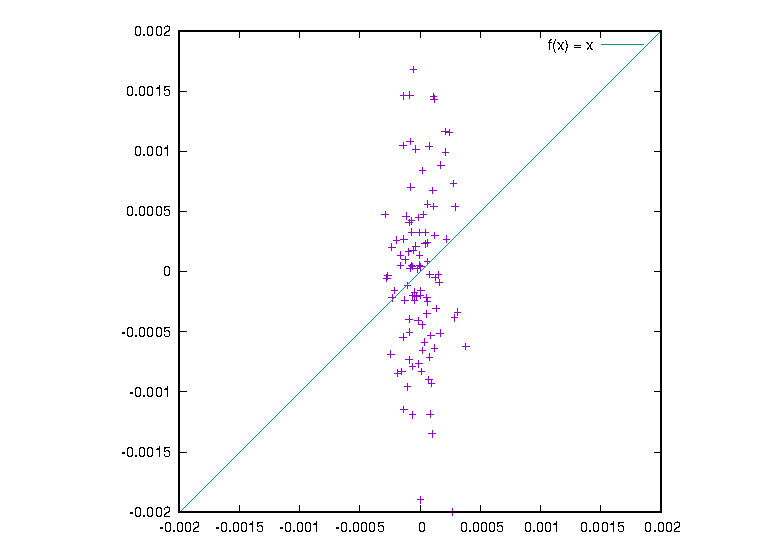
\includegraphics[scale=0.6]{./plots/rutile_72_scaled}};
  \node[below=of img1, node distance=0cm, yshift=1cm] {$E_{\text{classical} - \bar{E}_{\text{classical}}}$ (Ha/atom)};
  \node[left=of img1, node distance=0cm, rotate=90, anchor=center,yshift=-0.7cm] {$E_{\text{DFT}} - \bar{E}_{\text{DFT}}$ (Ha/atom)};
\end{tikzpicture}
\caption{DFT energy vs. classical energy (both shifted down by their average value) for 101 conformations of an $r-\text{TiO}_2$ lattice with 72 atoms.}
\label{rutile72}
\end{figure}

\begin{figure}[htb]
\begin{tikzpicture}
  \node (img1)  {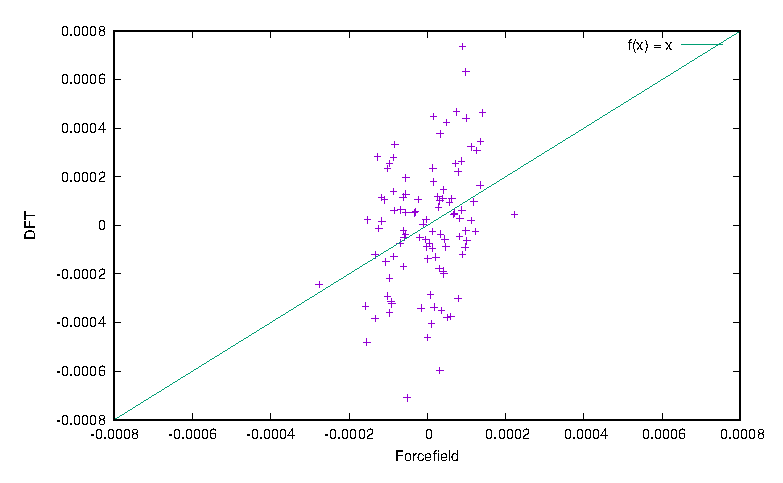
\includegraphics[scale=0.6]{./plots/nnp_198_scaled}};
  \node[below=of img1, node distance=0cm, yshift=1cm] {$E_{\text{classical} - \bar{E}_{\text{classical}}}$ (Ha/atom)};
  \node[left=of img1, node distance=0cm, rotate=90, anchor=center,yshift=-0.7cm] {$E_{\text{DFT}} - \bar{E}_{\text{DFT}}$ (Ha/atom)};
\end{tikzpicture}
\caption{DFT energy vs. classical energy (both shifted down by their average value) for 101 conformations of an $a-\text{TiO}_2$ nanoparticle with 198 atoms.}
\label{nnp_198}
\end{figure}

\tab Comparing the energies obtained using classical MD and those calculated using DFT reveals that a description of the forces inside an $a-\text{TiO}_2$ nanoparticle using only the two-body MA potential is not precise enough to yield an accurate representation of its potential energy surface (PES) (with respect to its atoms' positions).
Indeed, plotting the energies yielded by both calculation methods reveals that DFT calculation methods are much more sensitive to a change in a given nanoparticle's atomic configuration than classical methods.

\begin{figure}[htb]
\begin{tikzpicture}
  \node (img1)  {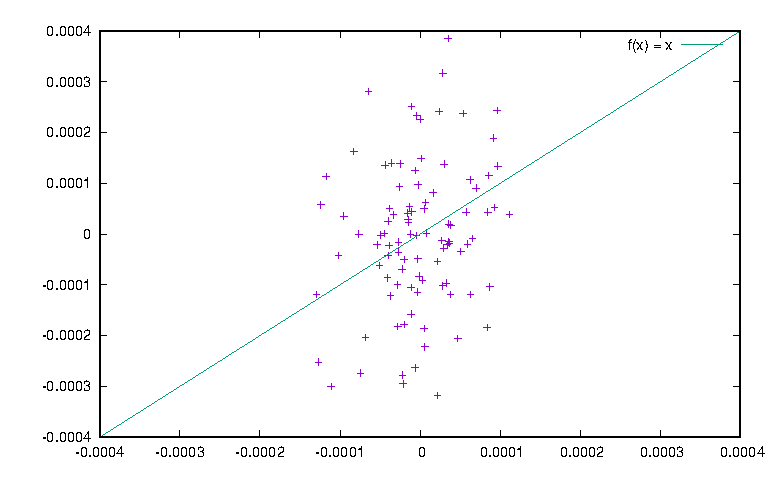
\includegraphics[scale=0.6]{./plots/nnp_390_scaled}};
  \node[below=of img1, node distance=0cm, yshift=1cm] {$E_{\text{classical} - \bar{E}_{\text{classical}}}$ (Ha/atom)};
  \node[left=of img1, node distance=0cm, rotate=90, anchor=center,yshift=-0.7cm] {$E_{\text{DFT}} - \bar{E}_{\text{DFT}}$ (Ha/atom)};
\end{tikzpicture}
\caption{DFT energy vs. classical energy (both shifted down by their average value) for 101 conformations of an $a-\text{TiO}_2$ nanoparticle with 390 atoms.}
\label{nnp_390}
\end{figure}

\tab The system for which this is the most obvious is the 768 atom nanoparticle, for which all classically evaluated energies lie within $\sim 10^{-4}\,\text{Ha}$ of each other, while the energies obtained usinq quantum mechanical methods vary by $\sim 10^{-1}\,\text{Ha}$.
One can get a sense of how dramatic this disparity between the ranges of of both data sets by examining figure \ref{nnp_768}: when plotting the DFT and classical data on the same scale, the classical energy values almost all lie on the same vertical line and thus appear to all be identical. 
While this effect is most dramatic for the 768 atom system, every other nanoparticle on which we ran similar calculations exhibit significant clustering of the energies obtained using the MA potential about their mean value, while their DFT energies spread out over a much larger interval.

\begin{figure}[htb]
\begin{tikzpicture}
  \node (img1)  {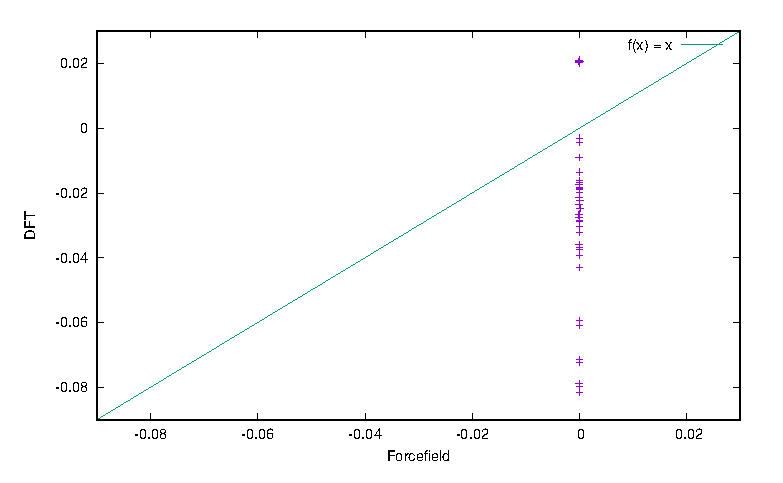
\includegraphics[scale=0.6]{./plots/nnp_768_fully_scaled}};
  \node[below=of img1, node distance=0cm, yshift=1cm] {$E_{\text{classical} - \bar{E}_{\text{classical}}}$ (Ha/atom)};
  \node[left=of img1, node distance=0cm, rotate=90, anchor=center,yshift=-0.7cm] {$E_{\text{DFT}} - \bar{E}_{\text{DFT}}$ (Ha/atom)};
\end{tikzpicture}
\caption{DFT energy vs. classical energy (both shifted down by their average value) for 101 conformations of an $a-\text{TiO}_2$ nanoparticle with 768 atoms.}
\label{nnp_768}
\end{figure}
  
\tab All four nanoparticles we ran these calculations exhibit weak correlation between the DFT-calculated energy values and the energies obtained using the MA potential. 
Even more surprisingly we find that the two sets of energy values of the different conformations of the rutile lattice were even less correlated than the ones obtained from the amorphous nanoparticles. 
Indeed, as can be seen in table \ref{stats}, our simulated rutile lattice yielded the lowest value of $\rho$ of all the systems we studied.

\begin{figure}[htb]
\begin{tikzpicture}
  \node (img1)  {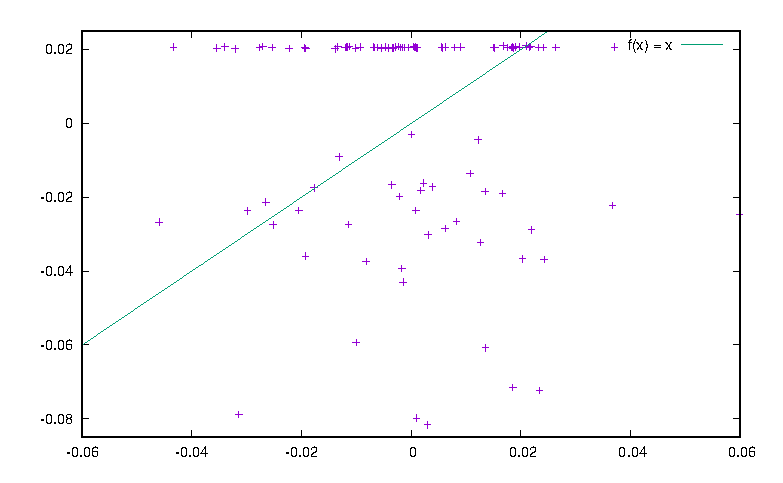
\includegraphics[scale=0.6]{./plots/nnp_768_dilated}};
  \node[below=of img1, node distance=0cm, yshift=1cm] {$500\cdot (E_{\text{classical} - \bar{E}_{\text{classical}})}$ (Ha/atom)};
  \node[left=of img1, node distance=0cm, rotate=90, anchor=center,yshift=-0.7cm] {$E_{\text{DFT}} - \bar{E}_{\text{DFT}}$ (Ha/atom)};
\end{tikzpicture}
\caption{Rescaled version of figure \ref{nnp_768}.}
\label{nnp_768d}
\end{figure}

In light of this extremely low correlation, we obviously cannot consider our simulated $r-\text{TiO}_2$ lattice a reference system. 
However this is not overly problematic, it simply suggests that a purely classical two-body description of atomic interactions in $\text{TiO}_2$ in the amorphous or rutile phase is not sufficiently accurate to keep track of small changes in the system's configuration.
Moreover the small RMSE values we get for all systems (except the 768-atom nanoparticle) and the fact that all classically obtained energies for a given system are very close to each other suggest that they are still physically sound at a less precise level of analysis.
Indeed, if both sets of energy values for each system varied over intervals of similar sizes and yet remained as uncorrelated as we have observed them to be, then the validity of trying to describe $\text{TiO}_2$ using only the MA potential would be seriously questioned.
However this is not the case; for every system all energies computed classically differ very little.
This is consistent with the fact that the atomic configurations from which such energies are computed were obtained from segments of our MD simulations where the system was already at equilibrium with its environment (i.e. the thermal bath) and thus did not vary greatly either.
It is therefore reassuring to see that, within our classical MD simulation, snapshots which have similar structures are also predicted to have close energy values. 
The contrast between the highly clustered classical values and the much more spread out quantum values could therefore suggest that the quantum description of $\text{TiO}_2$ is much more sensitive to the system's conformational changes while using the MA potential cannot meaningfully register such changes yet still provides an internally consistent and physically viable picture of the system.

[UNPHYSICAL CONFORMATIONS --> INCORRECT DFT RESULTS?]

\begin{table*}[]
\begin{tabular}{c|c|c|c|c}
System & $a-\text{TiO}_2$ (198 atoms) & $a-\text{TiO}_2$ (390 atoms) & $a-\text{TiO}_2$ (768 atoms)  & $r-\text{TiO}_2$ (72 atoms) \\ \hline
$\rho$ & 0.3066474                    & 0.3497706                    & -0.0496755                   & 0.0141203                   \\
RMSE   & 0.0486056                    & 0.0628487                    & 22.21090                       & 0.0518275                   \\
\end{tabular}
\label{stats}
\caption{Pearson correlation coefficient $\rho$ and RMSE between the energy values obtained through DFT and those obtained using the two-body MA potential on various configurations of different systems.}
\end{table*}

\tab Another possible explanation for the uncorrelatedness of the $r-\text{TiO}_2$ energy sets is our simulated lattice's small size.
As previously stated, the MA potential was developed to reproduce the bulk structures of $\text{TiO}_2$ in its various crystalline forms; the potential was developed by simulating nanocrystals ranging from 384 atoms to 576 atoms in size and the bulk properties of the different crystalline polytypes of titania were used to fix its energy parameters.
Knowing that the surface sites of a $\text{TiO}_2$ nanoparticle (crystalline or amorphous) have significantly different atomic and electronic structures as bulk sites\cite{vvh1,realistic_nnp,vvh2}, it is easy to see how a model built to simulate systems containing mainly bulk sites can reach erroneous results when trying reproduce a nanoparticle with a significant portion of its atoms on the surface.
A classical MD simulation of a larger $r-\text{TiO}_2$ lattice would probably yield a better set of reference conformation and energy values.
[BUT DFT = TOO EXPENSIVE]
Regardless of how well the MA potential describes $r-\text{TiO}_2$, the data we obtained from modeling amorphous systems unequivocally indicates that the MA potential is not accurate enough to reproduce their PES adequately. 

%\begin{table*}[]
%\begin{tabular}{c|c|c|c|c|c}
%System & $a-\text{TiO}_2$ (198 atoms) & $a-\text{TiO}_2$ (390 atoms) & $a-\text{TiO}_2$ (768 atoms) & $a-\text{TiO}_2$ (1842 atoms) & $r-\text{TiO}_2$ (72 atoms) \\ \hline
%$\rho$ & 0.3066474                    & 0.3497706                    & -0.0496755                   & TBC                           & 0.0141203                   \\
%RMSE   & 0.0486056                    & 0.0628487                    & 22.21090                     & TBC                           & 0.0518275                   \\
%\end{tabular}
%\label{stats}
%\caption{Pearson correlation coefficient $\rho$ and RMSE between the energy values obtained through DFT and those obtained using the two-body MA potential on various configurations of different systems.}
%\end{table*}

%\subsection{Comparing ALMO DFT with KS DFT}
 
%[FURTHER DISCUSSION: unshifted DFT values are ~500times larger than unshifted classical values rescale shifted energy values by dividing by average E?] 
 
\section*{Conclusion}

%\tab This paper's main objective was to quantify the accuracy of a simulation of amorphous titania nanoparticles using classical formalism.
%Using a set of common atomic configuration, we compared energy values obtained $\textit{via}$ a DFT calculation and those obtained using the classical MA potential, for $a-\text{TiO}_2$ nanoparticles of different sizes.
%All of the systems we simulated showed weak correlation between the classical and DFT energy values.

\tab Our comparison of the energy values we obtained through DFT and those calculated with the classical MA potential, on common sets of conformations of various $\text{TiO}_2$ nanoparticles has consistently revealed that these two data sets are weakly correlated.
Having established our DFT results to be more accurate than the ones yielded by the MA potential, we can safely assume that the MA potential does not faithfully reproduce the PES of small titania nanoparticles.
This holding true even for the set of energies obtained from a system which we believed to be well-described by both methods -- a 72-atom rutile nanocrystal -- raises some questions about our results and calls for further research into this topic:
\begin{itemize}
\item Are surface sites responsible for the disagreement between our energy values for $r-\text{TiO}_2$?
\item How necessary is the additional detail provided by DFT calculations to derive meaningful results from simulations of $\text{TiO}_2$ nanoparticles? 
\end{itemize}
These problems left unsolved call for further research into this topic; we examine certain possible ways in which the answers to the question posed here can be further elucidated.

%\tab Assuming that DFT calculations are necessary to properly sample from an $a-\text{TiO}_2$ nanoparticle's PES, we are now faced with the problem posed by the computing power necessary to run such calculations on large systems (i.e. nanoparticles containing more than $\sim\,$1000 atoms).
\tab Conducting a similar study on larger nanoparticles could provide further insight.
Indeed, the structure and properties of large nanoparticles are less impacted by their surface sites than smaller nanoparticles\cite{}
Seeing as computational expense is one of DFT's main drawbacks, a number of optimisation schemes have been proposed over the years to reduce both the amount of memory and the time necessary to run calculations on large systems ($\sim 1000$ atoms).
Among them, the absolutely localised molecular orbitals\cite{almo} (ALMO) method partitions the simulated system into small fragments (usually these are the individual atoms or molecules that compose it) and runs traditional DFT on each fragment in parallel.
This has the advantage of having a runtime that scales linearly with the number of fragments for large systems, while traditional DFT calculation runtimes scale cubically with the number of atoms being simulated.
Seeing as ALMO DFT makes a number of large DFT calculations much more feasible, it would allow us to conduct a similar study on larger nanoparticles (with more bulk sites) which could potentially yield better correlated classical and DFT values.
This could furthermore enable us to run simulations of nanoparticles with sizes closer to those of $a-\text{TiO}_2$ nanoparticles used in most practical applications ($\sim 4\,$nm\cite{realistic_nnp}) and therefore give us a better appreciation of how the MA potential performs on systems it is better adapted to model.

\tab Another way to run similar calculations on larger $\text{TiO}_2$ nanoparticles would be use smaller basis sets.
While the basis set we used to describe oxygen's electronic distribution (DZVP) cannot be further reduced without removing a polarisation function (which is crucial to adequately describe chemical bonding), the basis set we used for Ti explicitly describes the electrons in its three highest occupied subshells ($3p,\,3d,$ and $4s$).
Knowing that we can safely assume that titanum's six $3p$ elctrons have negligible impact on bonding in $\text{TiO}_2$, we can use a basis set and pseudopotential which treat them as core electrons.
This would significantly reduces the memory cost a DFT simulation of any system containing numerous Ti atoms, thus making DFT calculations on large $\text{TiO}_2$ nanoparticles more easily feasible.

[DISCUSSION OF SECOND QUESTION]

%\tab Having observed that DFT calculations are necessary to properly sample from an $a-\text{TiO}_2$ nanoparticle's PES, we are now faced with the problem posed by the computing power necessary to run such calculations on large systems (i.e. nanoparticles containing more than $\sim\,$1000 atoms).
%Seeing as computational expense is one of DFT's main drawbacks, a number of optimisation schemes have been proposed over the years to reduce both the amount of memory and the time necessary to run such calculations.
%Among them, we focus our attention to the absolutely localised molecular orbitals (ALMO) method which partitions the system being simulated into smaller fragments (usually these are the individual atoms or molecules that compose it) and runs traditional DFT on each fragment in parallel.
%This has the advantage of having a runtime that scales linearly with the number of fragments for large systems.
%Seeing as ALMO DFT makes a number of large DFT calculations much more feasible, we decide to test its accuracy on our various $a-\text{TiO}_2$ nanoparticles.
%As before, we evaluate the accuracy of the ALMO DFT method by comparing the energy it outputs for a given configuration of a nanoparticle with the energy obtained through classical DFT.  

$\bullet$ ALMO also needed to study size-dependence of certain properties (structural and electronic)

$\bullet$ Could also make large-nanoparticle simulations using smaller basis set for Ti. 

$\bullet$ Do a DFT MD simulation and re-calculate energies of equilibrated snapshots using MA potential: compare.

$\bullet$ Could also try using more elaborate (many-body) classical potential to do original MD run

%\textbf{Supporting Information}
%Calculated radial distribution functions of liquid water, comparison of timing benchmarks for the DZVP and TZV2P basis sets, timing benchmarks for systems containing 32,768 water molecules, timing benchmarks for the Kohn-Sham matrix build. This material is available free of charge via the Internet at http://pubs.acs.org.

%\textbf{Acknowledgments.} The research was funded by the Natural Sciences and Engineering Research Council of Canada through the Discovery Grant. The authors are grateful to Compute Canada and McGill HPC Centre for computer time.

\bibliography{tio2_nnp}

\end{document}
